\section{Design}

The design of the CND is a barrel, coaxial with the beamline, made of trapezoidal scintillator bars, read out via standard PMTs attached to long acrylic light guides. In order to optimize the light collection by matching the scintillator surface and the PMT entrance window, the detector is divided into 48 azimuthal segments and 3 radial layers, for a total of 24 blocks\footnote{A ``block'' or ``sector'' is formed by three radial layers of coupled pairs of scintillator bars.}, 144 scintillator bars, 144 PMTs, and 72 U-turn light guides (see Fig.~\ref{lab_CND_pic}). The radial thickness of all scintillators is 30 mm. The other dimensions are listed in Table~\ref{lab_scint_dim}.

\begin{figure}[htb]
  \centering
    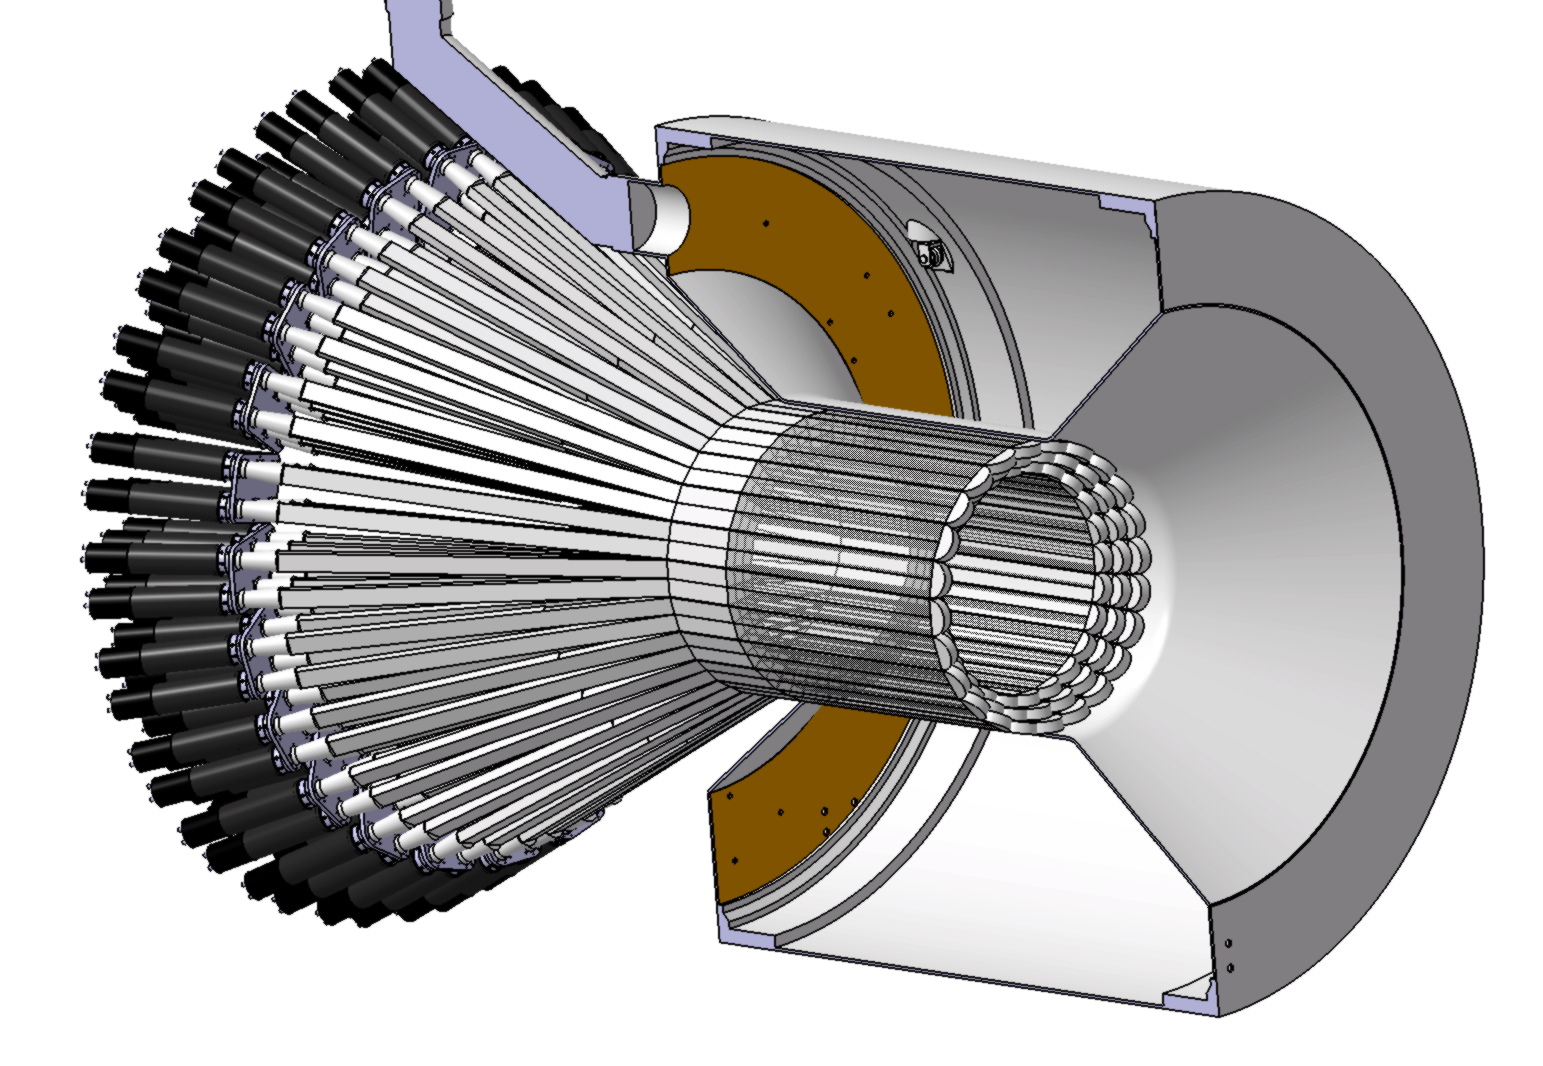
\includegraphics[width=0.45\textwidth]{Figure/CND_pic.jpg}
 \caption{Drawing of the CND inserted in the CLAS12 solenoid, which is shown in a cut-view.}
    \label{lab_CND_pic}
\end{figure}

\begin{table}[tbph]
\centering
\begin{tabular}{|c|c|c|c|c|}
\hline
Layer & Inner face & Outer face  & Length\\
 & width (mm) & width (mm) & (mm)\\
\hline
1 & 35.92 & 39.87 & 665.72 \\
2 & 40.0 & 43.95 & 700.0 \\
3 & 44.08 & 48.03 & 734.28 \\
\hline
\end{tabular}
\caption{Dimensions (mm) of the trapezoidal scintillator bars of the CND. The layer numbers go from the innermost (1) to the outermost (3). The thickness of all bars is 30 mm.}
\label{lab_scint_dim}

\end{table}
